\documentclass{article}

\usepackage[a4paper, total={6in, 8in}]{geometry}
\usepackage[utf8]{inputenc}
\usepackage{indentfirst}
\usepackage{graphicx}
\usepackage{textcomp}
\usepackage{colortbl}
\usepackage{siunitx}
\usepackage{multirow}
\usepackage{float} 

\usepackage{titlesec}
\setcounter{secnumdepth}{4}
\titleformat{\paragraph}{\normalfont\normalsize\bfseries}{\theparagraph}{1em}{}
\titlespacing*{\paragraph}{0pt}{3.25ex plus 1ex minus .2ex}{1.5ex plus .2ex}

\title{CS1237}

\begin{document}

\maketitle

\section{Chip Function Description}

The CS1237 is a high-precision, low-power analog-to-digital conversion chip with one differential 
input channel, built-in temperature sensor and high-precision oscillator.

The CS1237 PGA is optional: 1, 2, 64, 128. The default is 128.

CS1237 ADC data output rate in normal mode is optional: 10Hz, 40Hz, 640Hz, 1.28kHz, default is 10Hz;

The MCU can communicate with the CS1237 through the 2-wire SPI interface SCLK, $\overline{DRDY}$/DOUT to configure it, such as channel selection, PGA selection, output rate selection, and so on.

\subsection{The main function of the chip}

\begin{itemize}
    \item Built-in crystal
    \item Integrated temperature sensor
    \item With Power down function
    \item 2-wire SPI interface with a maximum speed of 1.1MHz

    \item 24 bits without missing code
\end{itemize}

\textbf{ADC functional characteristics:}

\begin{itemize}
    \item 24 bits without missing code
    \item PGA gain options: 1, 2, 64, 128
    \item One 24-bit differential input with no missing codes. When PGA=128 ENOB is 20 bits (5V),19.5 bits (3.3V)
    \item P-P noise: PGA=128, 10Hz: 180nV;
    \item INL less than 0.0015\%
    \item Output rate options: 10Hz, 40Hz, 640Hz, 1.28kHz
    \item In-band short function
\end{itemize}

\subsection{Chip applications}

\begin{itemize}
    \item Industrial process control
    \item Electronic scale
    \item Liquid/gas chemical analysis
    \item Blood meter
    \item Smart converter
    \item Portable equipment
\end{itemize}

\subsection{Chip basic structure function description}

The CS1237 is a high-precision, low-power Sigma-Delta analog-to-digital converter with one Sigma-Delta ADC, one differential input channel, and one temperature sensor. The ADC uses a two-stage sigma delta modulator through a low-noise instrumentation amplifier. To achieve PGA amplification, magnification options: 1, 2, 64, 128. At PGA=128, the effective resolution is up to 20 bits (working at 5V).

The CS1237 has an internal RC oscillator and does not require an external crystal.

The CS1237 can be configured for multiple functional modes via $\overline{DRDY}$/DOUT and SCLK, such as temperature detection, PGA selection, ADC data output rate selection, and more.

The CS1237 has Power down mode.

\begin{figure}[h]
    \centering
    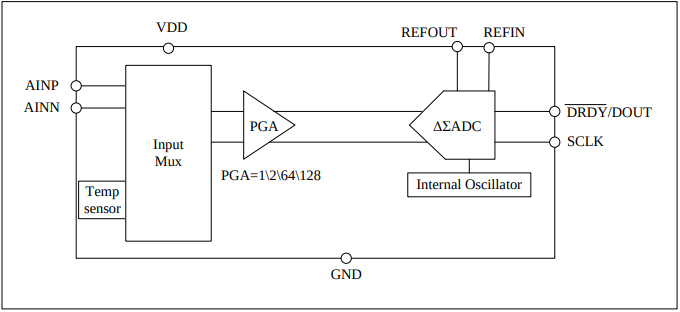
\includegraphics[width=1\textwidth]{fig1.png}
    \caption{CS1237 Functional Block Diagram}
    \label{fig:fig1}
\end{figure}

\pagebreak

\subsection{Absolute maximum limit of the chip}

\begin{table}[h]
    \makebox[\textwidth]{%
    \begin{tabular}{ |l|c|c|c|c| }
        \hline
        \rowcolor[gray]{0.8}
        \textbf{Name} & \textbf{Symbol} & \textbf{Minimal} & \textbf{Maximum} & \textbf{Unit} \\
        \hline
        Voltage & VDD  & -0.3 & 6 & V \\
        \hline
        Power instantaneous current & & & 100 & mA \\
        \hline
        Power supply constant current & & & 10 & mA\\
        \hline
        Digital pin input voltage & & -0.3 & DVDD+0.3 & V \\
        \hline
        Digital output pin voltage & & -0.3 & DVDD+0.3 & V \\
        \hline
        Temperature & & & 150 & \textdegree C \\
        \hline
        Operating temperature & & -40 & 85 & \textdegree C \\
        \hline
        Storage temperature & & -60 & 150 & \textdegree C \\
        \hline
        Chip pin soldering temperature & & & 240 & \textdegree C \\
        \hline
    \end{tabular}}
    \caption{CS1237 Limits}
    \label{tab:table1}
\end{table}

\subsection{CS1237 Digital Logic Features}

\begin{table}[h]
    \makebox[\textwidth]{%
    \begin{tabular}{ |l|c|c|c|c|c| }
        \hline
        \rowcolor[gray]{0.8}
        \textbf{Parameter} & \textbf{Minimal} & \textbf{Typical} & \textbf{Maximum} & \textbf{Unit} & \textbf{Condition Description} \\
        \hline
        VIH & 0.7xDVDD & & DVDD+0.1 & V & \\
        \hline
        VIL & DGND & & 0.3xDVDD & V & \\
        \hline
        VOH & DVDD-0.4 & & DVDD & V & Ioh=1mA\\
        \hline
        VOL & DGND & & 0.2xDVDD & V & IoL=1mA\\
        \hline
        IIH & & & 10 & $\mu$A & VI=DVDD\\
        \hline
        IIL & -10 & & & $\mu$A & VI=DVDD\\
        \hline
        Serial clock SCLK operating frequency & & & 1.1 & MHz & \\
        \hline
    \end{tabular}}
    \caption{CS1237 Digital Logic Features}
    \label{tab:table2}
\end{table}

\pagebreak

\subsection{CS1237 Electrical Characteristics}

All parameter tests are tested at ambient temperature -40 to 85°C with built-in reference conditions, unless
otherwise noted.

\begin{table}[h]
    \makebox[\textwidth]{%
    \begin{tabular}{ |l|c|c|c|c|c| }
        \hline
        \rowcolor[gray]{0.8}
        \textbf{Parameter} & \textbf{Condition} & \textbf{Min} & \textbf{Typical} & \textbf{Max} & \textbf{Unit} \\ 
        \hline
            \rowcolor[gray]{0.8}
            \multicolumn{6}{|l|}{\textbf{Analog input}} \\
        \hline
            Full-scale input voltage (AINP-AINN) & & & $\pm$0.5VREF/PGA & & V \\
        \hline
            \multirow{2}{*}{Common-mode input voltage} 
                & PGA=1,2 & AGND-0.1 & & AVDD+0.1 & V \\ \cline{2-6}
                & PGA=64,128 & AGND+0.75 & & AVDD-0.75 & V \\ 
        \hline
            \multirow{2}{*}{Differential input impedance} 
                & PGA=1,2 & & 190 & & M$\Omega$ \\ \cline{2-6}
                & PGA=64,128 & & 28 & & M$\Omega$\\
        \hline
            \rowcolor[gray]{0.8}
            \multicolumn{6}{|l|}{\textbf{System performance}}\\
        \hline
            Resolution & No missing code & & 24 & & Bits \\
        \hline
            AD rate & & & 10 & 1280 & Hz \\
        \hline
            \multirow{2}{*}{System performance} & \multirow{2}{*}{Full establishment} & \multicolumn{3}{c|}{3: ADC output rate is 10-40Hz,} & \multirow{2}{*}{Conversion Cycle} \\ 
            & & \multicolumn{3}{c|}{4: ADC output rate is 640-1280Hz} & \\
        \hline
            P-P noise & PGA=128,10Hz & & 180 & & nV \\
        \hline
            \multirow{2}{*}{Effective accuracy} & \multirow{2}{*}{PGA=128,10Hz} & \multirow{2}{*}{ } & 20(5V) & \multirow{2}{*}{ } & \multirow{2}{*}{Bit} \\
            & & & 19.5(3.3V) & & \\
        \hline
            Integral linearity & PGA=128 & & $\pm$15 & & pmm \\
        \hline
            Offset error & PGA=128 & & $\pm$1.4 & & $\mu$V \\
        \hline
            Offset error drift & PGA=128 & & 20 & & nV/\textdegree C \\
        \hline
            Gain error & PGA=128 & & $\pm$0.5 & & \% \\
        \hline
            Gain error drift & PGA=128 & & 8 & & ppm/\textdegree C \\
        \hline
            \rowcolor[gray]{0.8}
            \multicolumn{6}{|l|}{\textbf{Reference voltage input}} \\
        \hline 
            Reference voltage input & REFIN & 1.5 & VDD & VDD+0.1 & V \\
        \hline
            \rowcolor[gray]{0.8}
            \multicolumn{6}{|l|}{\textbf{Reference voltage output}} \\
        \hline 
            Reference voltage output & REFOUT & & VDD & & V \\
        \hline
            \rowcolor[gray]{0.8}
            \multicolumn{6}{|l|}{\textbf{Clock}} \\
        \hline
            Internal oscillator frequency & & & 5.2 & & MHz \\
        \hline
            Built-in clock drift & & & 250 & & ppm/\textdegree C \\
        \hline
            \rowcolor[gray]{0.8}
            \multicolumn{6}{|l|}{\textbf{Temperature Sensor}} \\
        \hline 
            Temperature measurement error & TempError & & $\pm$3 & & \textdegree C \\
        \hline
    \end{tabular}}
    \caption{CS1237 Electrical Characteristics (VDD = 5V, 3.3V)}
    \label{tab:table3}
\end{table}

\begin{table}[H]
    \makebox[\textwidth]{%
    \begin{tabular}{|l|c|c|c|c|c|c|}
        \hline
            \rowcolor[gray]{0.8}
            \textbf{Parameter} & \multicolumn{2}{|c|}{\textbf{Condition}} & \textbf{Min} & \textbf{Typical} & \textbf{Max} & \textbf{Unit} \\ 
        \hline 
            Voltage & \multicolumn{2}{|c|}{VDD} & 4.5 & 5 & 5.5 & V \\
        \hline
            \multirow{3}{*}{Working current} & \multirow{2}{*}{Normal Mode} & PGA=1,2 & & 1.57 & & mA \\ \cline{3-7}
            & & PGA=64,128 & & 2.34 & & mA \\ \cline{2-7}
            & \multicolumn{2}{|c|}{Power Down} & & 0.1 & 0.1 & $\mu$A \\
        \hline
    \end{tabular}}
    \caption{CS1237 Power Supply Electrical Characteristics (VDD=5V)}
    \label{tab:table4}
\end{table}

\begin{table}[H]
    \makebox[\textwidth]{%
    \begin{tabular}{|l|c|c|c|c|c|c|}
        \hline
            \rowcolor[gray]{0.8}
            \textbf{Parameter} & \multicolumn{2}{|c|}{\textbf{Condition}} & \textbf{Min} & \textbf{Typical} & \textbf{Max} & \textbf{Unit} \\ 
        \hline 
            Voltage & \multicolumn{2}{|c|}{VDD} & 3 & 3.3 & 3.6 & V \\
        \hline
            \multirow{3}{*}{Working current} & \multirow{2}{*}{Normal Mode} & PGA=1,2 & & 1.26 & & mA \\ \cline{3-7}
            & & PGA=64,128 & & 2.11 & & mA \\ \cline{2-7}
            & \multicolumn{2}{|c|}{Power Down} & & 0.1 & & $\mu$A \\
        \hline
    \end{tabular}}
    \caption{CS1237 Power Supply Electrical Characteristics (VDD=3.3V)}
    \label{tab:table5}
\end{table}

\subsection{Chip pin}

\begin{figure}[h]
    \centering
    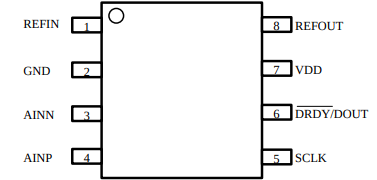
\includegraphics[width=0.5\textwidth]{fig2.png}
    \caption{CS1237 Chip Pinout}
    \label{fig:fig2}
\end{figure}

\begin{table}[h]
    \makebox[\textwidth]{%
    \begin{tabular}{|l|c|c|c|}
        \hline
            \rowcolor[gray]{0.8}
            \textbf{No.} & \textbf{Pin Name} & \textbf{Input/Output} & \textbf{Instructions} \\ 
        \hline 
            1 & REFIN & AI & Reference source input \\
        \hline
            2 & GND & P & Chip ground \\
        \hline
            3 & AINN & AI & Channel negative input \\
        \hline
            4 & AINP & AI & Channel positive input \\
        \hline
            5 & SCLK & DI & SPI input interface \\
        \hline
            6 & $\overline{DRDY}$/DOUT & DI/DO & SPI data input-output interface \\
        \hline
            7 & VDD & P & power supply \\
        \hline
            8 & REFOUT & AO & Reference output \\
        \hline
    \end{tabular}}
    \caption{Note: REFOUT is the sensor excitation source output (output value is VDD).}
    \label{tab:table6}
\end{table}

\pagebreak

\section{Chip Function Module Description}

\subsection{Analog input front end}

There is one ADC in CS1237, one differential input is integrated. The signal input can be differential
input signal AINP, AINN, or the output signal of temperature sensor. The switching of input signal is
controlled by register (ch\_sel[1:0]). The basic structure is shown below:

\begin{figure}[h]
    \centering
    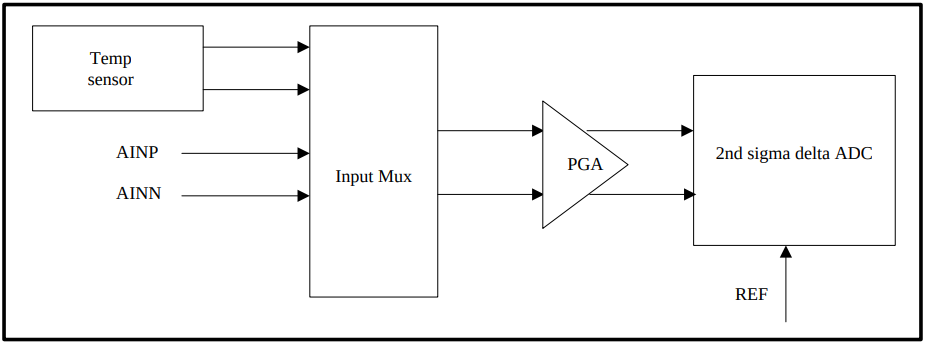
\includegraphics[width=1\textwidth]{fig3.png}
    \caption{Analog input structure diagram}
    \label{fig:fig4}
\end{figure}

The CS1237 PGA can be configured with: 1, 2, 64, 128, controlled by registers (pga\_sel[1:0]);

The reference voltage can be either external or internal. If an external reference voltage is to be used,
the internal reference must be turned off first and the internal reference control is controlled by a
register (refo\_off).

\subsection{Temperature Sensor}

The chip provides temperature measurement inside. When ch\_sel[1:0]=2'b10, the ADC analog signal input is
connected to the internal temperature sensor, and other analog input signals are invalid. The ADC derives
the actual temperature value by measuring the voltage difference at the output of the internal
temperature sensor. When ch\_sel[1:0]=2’b10, ADC only supports PGA=1. \textbf{The temperature sensor
requires a single point of correction. Correction method: At a certain temperature point A, a temperature
sensor is used to measure the code value Ya.} 

\textbf{Then the temperature of other temperature point: }

\begin{equation}
B = \frac{Yb*(273.15 + A)}{Ya-273.15}
\end{equation}

\textbf{A is the temperature unit is Celsius. Ya is the A-point corresponding temperature code value. 
Yb is the temperature code value corresponding to point B.}

\pagebreak

\subsection{Low noise PGA amplifier}

CS1237 provides a low-noise, low-drift PGA amplifier and bridge sensor differential output connection,
the basic structure of the diagram as shown below, front anti-EMI filter circuit R = 450$\Omega$, C = 18pF 20M
high-frequency filtering.
The low-noise PGA amplifier achieves 64-fold amplification with RF1, R1, RF2, and PGA amplification with
64- and 128-point PGA.
Different PGAs such as 1, 2, 64, and 128 are configured through pga\_sel[1:0].
When using PGA = 1,2, the 64-times low-noise PGA amplifier is turned off to save power.
When using a low-noise PGA amplifier, the input range is between GND + 0.75V and VDD - 0.75V. 
Exceeding this range results in a decrease in actual performance.
Connect a built-in 45pF capacitor at the CAP port, and make a low-pass filter with the built-in 2k
resistor RINT to use as a high-frequency filter for the output signal of the low-noise PGA amplifier. 
The low-pass filter can also be used as an anti-alias filter for the ADC.

\begin{figure}[h]
    \centering
    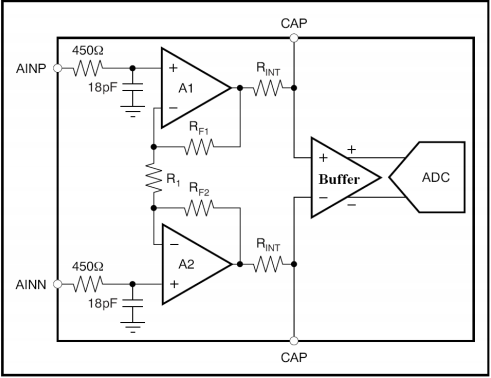
\includegraphics[width=1\textwidth]{fig4.png}
    \caption{PGA structure diagram}
    \label{fig:fig4}
\end{figure}

CS1237 has built-in buffer. 
When PGA=1,2, CS1237 uses Buffer to reduce problems caused by low ADC differential input impedance, such
as insufficient settling time and large gain error. 
When PGA=64,128, CS1237 also Use Buffer to reduce setup error, gain error, and inner code drift caused by
the low-pass filtering of low noise PGA with RINT=2K, CINT=0.1$\mu$F.

\subsection{Clock source}

The CS1237 uses a built-in crystal to provide the system's desired clock frequency, typically 5.2MHz.

\subsection{Reset and power off(POR \& power down)}

When the chip is powered on, the built-in power-on reset circuit will generate a reset signal to
automatically reset the chip.

When SCLK goes from low to high and stays high for more than 100$\mu$s, the CS1237 enters PowerDown mode,
which consumes less than 0.1$\mu$A. When SCLK goes back low, the chip will resume normal operation.

When the system is re-entered into normal working mode by Power down, all functions are configured to be in the state before Power Down, and no functional configuration is required.

\pagebreak

\subsection{SPI serial communication}

2-wire SPI serial communication is used in the CS1237, and data reception and function configuration can be realized through SCLK and $\overline{DRDY}$/DOUT.

\subsubsection{Setup time}

When the ADC data output rate is 10Hz or 40Hz, the digital part needs to have 3 data conversion periods to meet the establishment of the analog input signal and the filter settling time requirement; When the ADC data output rate is 640Hz or 1280Hz, the digital part needs to have 4 data conversion cycles to meet the setup of the analog input signal and the settling time of the filter. The entire setup process of CS1237 is shown in the following figure:

\begin{figure}[h]
    \centering
    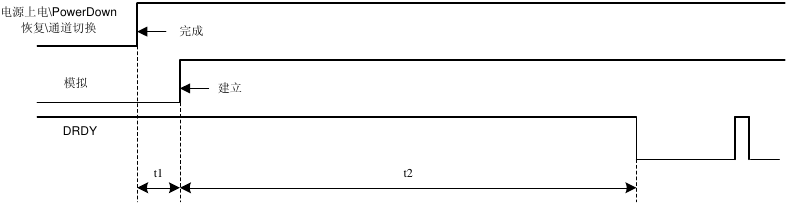
\includegraphics[width=1\textwidth]{fig5.png}
    \caption{Data Creation Process 1}
    \label{fig:fig5}
\end{figure}

\begin{figure}[h]
    \centering
    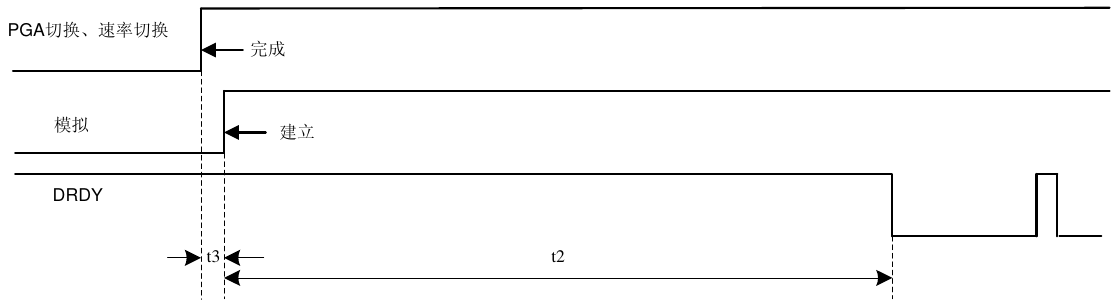
\includegraphics[width=1\textwidth]{fig6.png}
    \caption{Data Creation Process 2}
    \label{fig:fig6}
\end{figure}

\begin{table}[h]
    \makebox[\textwidth]{%
    \begin{tabular}{|c|l|c|c|c|c|c|}
        \hline
            \rowcolor[gray]{0.8}
            \textbf{Parameter} & \multicolumn{2}{|c|}{\textbf{Description (1)}} & \textbf{Minimum value} & \textbf{Typical value} & \textbf{Maximum} & \textbf{Unit} \\ 
        \hline 
            \multirow{2}{*}{t1} & \multicolumn{2}{|l|}{Power On/Power Down Recovery/Setting time} &  & \multirow{2}{*}{2} &  & \multirow{2}{*}{ms}\\
             & \multicolumn{2}{|c|}{required for simulation after channel switching} & & & & \\
        \hline
            \multirow{2}{*}{t3} & \multicolumn{2}{|l|}{Settling time required for simulation after PGA}  &  & \multirow{2}{*}{0.8} &  & \multirow{2}{*}{$\mu$s} \\
            & \multicolumn{2}{|l|}{switch/rate switching} & & & & \\
        \hline
            \multirow{2}{*}{t2} & Setting time ($\overline{DRDY}$/DOUT & 10/40Hz &  & 300/75 &  & ms\\
            \cline{3-7}
             & remains high) & 640/1280Hz &  & 6.25/3.125 &  & ms\\
        \hline
    \end{tabular}}
    \label{tab:tableX}
\end{table}

\subsubsection{ADC data output rate}

The CS1237 data output rate can be configured via the registers speed\_sel[1:0].

\begin{table}[h]
    \makebox[\textwidth]{%
    \begin{tabular}{|c|c|}
        \hline
            \rowcolor[gray]{0.8}
            \textbf{SPEED\_SEL[1:0]} & \textbf{ADC output rate (Hz)} \\ 
        \hline 
            00 & 10\\
        \hline
            01 & 40\\
        \hline
            10 & 640\\
        \hline
            11 & 1280\\
        \hline
    \end{tabular}}
    \caption{Output Rate Settings}
    \label{tab:table7}
\end{table}

\subsubsection{Data Format}

The data output by CS1237 is 24-bit 2's complement, and the highest bit (MSB) is the first output.
The least significant bit (LSB) is (0.5VREF/Gain)/($2^{23}$-1).
The positive full-size output code is 7FFFFFH, and the negative full-size output code is 800000H.
The table below shows the ideal output codes for the different analog input signals.

\begin{table}[h]
    \makebox[\textwidth]{%
    \begin{tabular}{|c|c|}
        \hline
            \rowcolor[gray]{0.8}
            \textbf{Input signal VIN (AINP-AINN)} & \textbf{Ideal output} \\ 
        \hline 
            $\geq$+0.5VREF/Gain & 7FFFFFH \\
        \hline
            (+0.5VREF/Gain)/($2^{23}$ -1) & 000001H \\
        \hline
            0 & 000000H \\
        \hline
            (-0.5VREF/Gain)/($2^{23}$ -1) & FFFFFFH \\
        \hline
            $\leq$+0.5VREF/Gain & 800000H \\
        \hline
    \end{tabular}}
    \caption{Ideal output code and input signal (1)}
    \label{tab:table7}
\end{table}

(1) Regardless of noise, INL, offset error and gain error

\subsubsection{Data preparation, data input and output ($\overline{DRDY}$/DOUT)}

The $\overline{DRDY}$/DOUT pin has 4 uses.
First, when the output is low, it means that the new data has been converted;
Second, as the data output pin, when the data is ready, after the rising edge of the first SCLK, $\overline{DRDY}$/DOUT outputs the highest bit (MSB) of the converted data.
On each rising edge of SCLK, the data is automatically shifted by one bit.
Reads all 24-bit data after 24 SCLKs. 
If SCLK is paused at this time, $\overline{DRDY}$/DOUT will hold the last bit of data until the next data is ready to be pulled high, after which $\overline{DRDY}$/DOUT is Pulling low again, indicating that the new data has been converted, and the next data can be read;
Fourth, as the register data write or read pin, when the configuration register or read register value is needed, the SPI needs to send 46 SCLKs. 
According to the command word input by $\overline{DRDY}$/DOUT, it is judged whether it is a write register operation or a read register operation. .

\subsubsection{Serial clock input (SCLK)}

Serial Clock Input SCLK is a digital pin.
This signal should be guaranteed to be a clean signal, and glitch or slow rising edges can cause errors or errors to be read.
Therefore, it should be ensured that the rise and fall times of SCLK are less than 50ns.

\subsubsection{Data transmission}

The CS1237 can continuously convert the analog input signal. When $\overline{DRDY}$ /DOUT is pulled low, it indicates that the data is ready to be accepted. 
The first SCLK input can read the highest bit of the output. 
After 24 SCLKs, all the signals will be read. 24-bit data read. 
If SCLK is suspended, $\overline{DRDY}$/DOUT will hold the last bit of data until it is pulled high.
Whether the 25th and 26th SCLK output configuration registers have a write flag, the $\overline{DRDY}$/DOUT corresponding to the 25th SCLK is 1 indicating that the configuration register Config has been written with a new value.
The $\overline{DRDY}$/DOUT corresponding to the 26th SCLK is the chip extension reserved bit, and the current output is always 0.
$\overline{DRDY}$/DOUT can be pulled high by the 27th SCLK, and then $\overline{DRDY}$/DOUT is pulled low again, indicating that the new data is ready to be accepted and the next data is converted.
The basic timing is shown in the figure:

\begin{figure}[h]
    \centering
    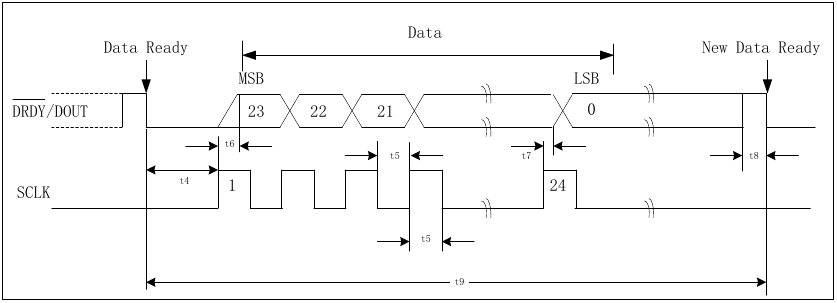
\includegraphics[width=1\textwidth]{fig7.png}
    \caption{Read data timing diagram 1}
    \label{fig:fig7}
\end{figure}

\begin{figure}[h]
    \centering
    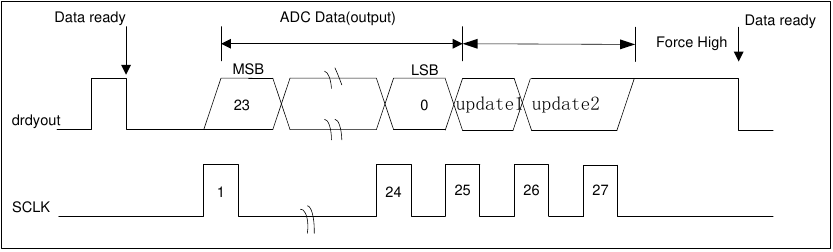
\includegraphics[width=1\textwidth]{fig8.png}
    \caption{Read data timing diagram 2}
    \label{fig:fig8}
\end{figure}

\begin{table}[h]
    \makebox[\textwidth]{%
    \begin{tabular}{|c|c|c|c|c|c|c|}
        \hline
            \rowcolor[gray]{0.8}
            \textbf{SYMBOL} & \multicolumn{2}{|c|}{\textbf{DESCRIPTION}} & \textbf{MIN} & \textbf{TYP} & \textbf{MAX} & \textbf{UNITS} \\
        \hline 
            t4 & \multicolumn{2}{|l|}{$\overline{DRDY}$/DOUT goes low to the first SCLK rising edge} & 0 & & & ns\\
        \hline
            t5 & \multicolumn{2}{|l|}{SCLK high or low pulse width} & 455 & & & ns \\
        \hline
            t6 & \multicolumn{2}{|l|}{SCLK rising edge to new data bit valid (transmission delay)} & 455 & & & ns \\
        \hline
            t7 & \multicolumn{2}{|l|}{SCLK rising edge to old data bit valid (hold time)} & 227.5 & & 455 & ns \\
        \hline
            t8 & \multicolumn{2}{|l|}{Data update, not allowed to read previous data} & & 26.13 & & $\mu$s \\
        \hline
            \multirow{4}{*}{t9} & \multirow{4}{*}{Conversion time (1/data rate)} & 10Hz& & 100 & & ms\\
        \cline{3-7}
            & & 40Hz& & 25& & ms\\
        \cline{3-7}
            & & 640Hz& & 1.5625 & & ms\\
        \cline{3-7}
            & & 1280Hz& & 0.78125 & & ms\\
        \hline 
    \end{tabular}}
    \caption{Read data timing table}
    \label{tab:table9}
\end{table}

\subsubsection{Functional configuration}

The CS1237 can be configured with different functions through SCLK and $\overline{DRDY}$/DOUT. 
The function configuration timing diagram is shown below:

\begin{figure}[h]
    \centering
    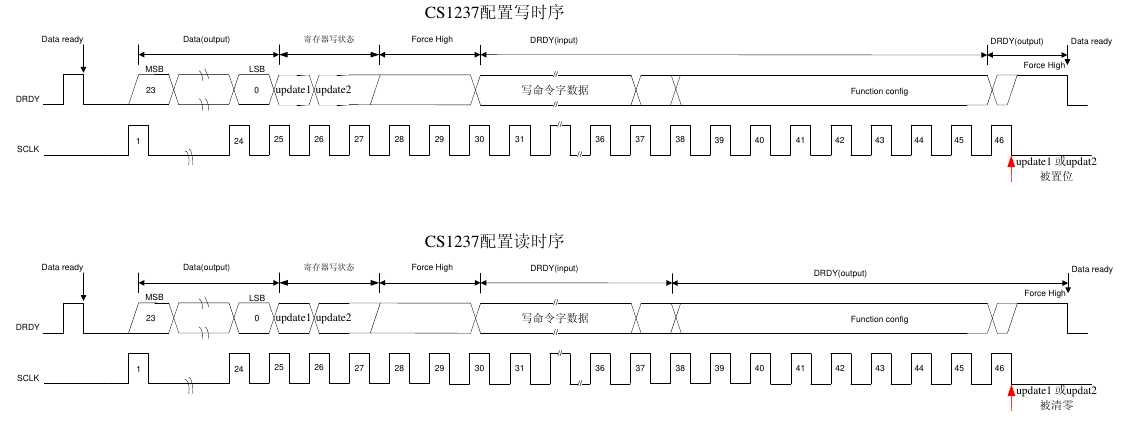
\includegraphics[width=1\textwidth]{fig9.png}
    \caption{Function configuration timing diagram}
    \label{fig:fig9}
\end{figure}

A brief description of the functional configuration process, after $\overline{DRDY}$/DOUT goes from high to low:

\begin{enumerate}
    \item The 1st to 24th SCLKs read the ADC data. If you do not need to configure registers or read registers, you can omit the following steps.
    \item The 25th to 26th SCLKs read the register write operation status.
    \item The 27th SCLK pulls the $\overline{DRDY}$/DOUT output high.
    \item From the 28th to the 29th SCLK, switch $\overline{DRDY}$/DOUT to the input.
    \item The 30th to 36th SCLK, the input register writes or reads the command word data (the high order first input).
    \item The 37th SCLK, the direction of $\overline{DRDY}$/DOUT is switched (if it is a write register, $\overline{DRDY}$/DOUT is the input; if it is a read register, $\overline{DRDY}$/DOUT is the output).
    \item The 38th to 45th SCLK, input register configuration data or output register configuration data (high order first input/output).
    \item For the 46th SCLK, switch $\overline{DRDY}$/DOUT to the output and pull $\overline{DRDY}$/DOUT high. Update1/update2 is set or cleared.
\end{enumerate}

\paragraph{SPI command word}

CS1237 has 2 command words, the length of the command word is 7bits, and the command words are described as follows:

\begin{table}[h]
    \makebox[\textwidth]{%
    \begin{tabular}{|c|c|c|}
        \hline
            \rowcolor[gray]{0.8}
            \textbf{Command name} & \textbf{Command byte} & \textbf{Description} \\ 
        \hline 
            Write configuration register & 0x65 & Write configuration register Config \\
        \hline
            Read configuration register & 0x56 & Read configuration register Config \\
        \hline
    \end{tabular}}
    \caption{Command word description table}
    \label{tab:table10}
\end{table}

\pagebreak

\paragraph{SPI register}

The CS1237 has a set of Config registers.

\begin{table}[h]
    \makebox[\textwidth]{%
    \begin{tabular}{|c|c|c|c|}
        \hline
            \rowcolor[gray]{0.8}
            \textbf{Register} & \textbf{R/W} & \textbf{Description} & \textbf{Reset value} \\ 
        \hline 
            Description & Reserved bit & Configuration register & 0x0C \\
        \hline
    \end{tabular}}
    \label{tab:tableaux1}
\end{table}

\begin{table}[h]
    \makebox[\textwidth]{%
    \begin{tabular}{|c|c|c|c|c|}
        \hline
            \rowcolor[gray]{0.8}
            \textbf{Configuration bit} & \textbf{B7} & \textbf{B6} & \textbf{B5} & \textbf{B4} \\ 
        \hline 
            Description & Reserved bit & REF output switch & \multicolumn{2}{|c|}{ADC output rate selection} \\
        \hline
            \rowcolor[gray]{0.8}
            \textbf{Configuration bit} & \textbf{B3} & \textbf{B2} & \textbf{B1} & \textbf{B0} \\ 
        \hline 
            Description &  \multicolumn{2}{|c|}{PGA selection} &  \multicolumn{2}{|c|}{Channel selection}  \\
        \hline
    \end{tabular}}
    \label{tab:tableaux2}
\end{table}

\begin{table}[h]
    \makebox[\textwidth]{%
    \begin{tabular}{|c|c|c|c|}
        \hline
            \rowcolor[gray]{0.8}
            \textbf{Bits} & \multicolumn{3}{|l|}{\textbf{Description}} \\ 
        \hline 
            [7] & - & \multicolumn{2}{|l|}{The chip retains the use bits. \textbf{The default is 0, write 0 when writing, do not write 1}} \\
        \hline 
            \multirow{3}{*}{[6]} & \multirow{3}{*}{REFO\_OFF} & \multicolumn{2}{|l|}{\textbf{REF output switch:} Default REF output is on} \\
            & & \multicolumn{2}{|l|}{1 = Turn off REF output.} \\
            & & \multicolumn{2}{|l|}{0 = REF Normal output.} \\
        \hline 
            \multirow{6}{*}{[5:4]} & \multirow{6}{*}{SPEED\_SEL} & \multicolumn{2}{|l|}{\textbf{ADC output rate selection:}The default is 10Hz} \\
            \cline{3-4}
                & & \textbf{SPEED\_SEL[1:0]} & \textbf{Description} \\
            \cline{3-4}
                & & 00 & ADC output rate is 10Hz \\
            \cline{3-4}
                & & 01 & ADC output rate is 40Hz \\
            \cline{3-4}
                & & 10 & ADC output rate is 640Hz \\
            \cline{3-4}
                & & 11 & ADC output rate is 1280Hz \\
        \hline 
            \multirow{6}{*}{[3:2]} & \multirow{6}{*}{PGA\_SEL} & \multicolumn{2}{|l|}{\textbf{PGA selection:}The default PGA is 128, in the temperature mode PGA\_SEL=00} \\
            \cline{3-4}
                & & \textbf{PGA\_SEL[1:0]} & \textbf{Description} \\
            \cline{3-4}
                & & 00 & 1 \\
            \cline{3-4}
                & & 01 & 2 \\
            \cline{3-4}
                & & 10 & 64\\
            \cline{3-4}
                & & 11 & 128 \\
        \hline 
            \multirow{6}{*}{[1:0]} & \multirow{6}{*}{CH\_SEL} & \multicolumn{2}{|l|}{\textbf{Channel selection:}The default channel is channel A} \\
            \cline{3-4}
                & & \textbf{CH\_SEL[1:0]} & \textbf{Description} \\
            \cline{3-4}
                & & 00 & Channel A \\
            \cline{3-4}
                & & 01 & Chip retention \\
            \cline{3-4}
                & & 10 & Temperature \\
            \cline{3-4}
                & & 11 & Internal short \\
        \hline 
    \end{tabular}}
    \caption{Config register description table}
    \label{tab:table11}
\end{table}

\pagebreak

\subsubsection{Power down mode}

When SCLK goes from low to high and stays high for more than 100$\mu$s, CS1237 enters PowerDown mode, which will turn off all circuits of the chip, and the power consumption is close to 0.
When SCLK returns to low level, the chip will re-enter normal operation.

\begin{figure}[h]
    \centering
    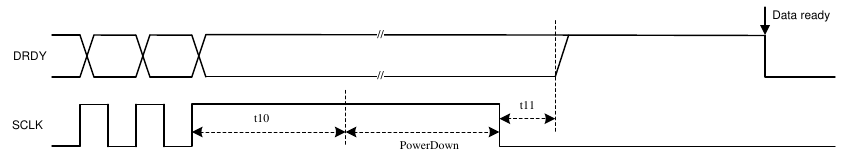
\includegraphics[width=1\textwidth]{fig10.png}
    \caption{PowerDown mode diagram}
    \label{fig:fig10}
\end{figure}

\begin{table}[h]
    \makebox[\textwidth]{%
    \begin{tabular}{|c|c|c|c|c|}
        \hline
            \rowcolor[gray]{0.8}
            \textbf{Symbol} & \textbf{Description} & \textbf{Minimum value} & \textbf{Typical value}  & \textbf{Maximum} \\ 
        \hline 
            t10 & SCLK high hold time & 100$\mu$s & & \\
        \hline
            t11 & Low hold time after SCLK falls & 10$\mu$s & & \\
        \hline
    \end{tabular}}
    \label{tab:finaltable}
\end{table}

\pagebreak

\section{Chip package}

CS1237 is available in SOP8 package.

\begin{figure}[h]
    \centering
    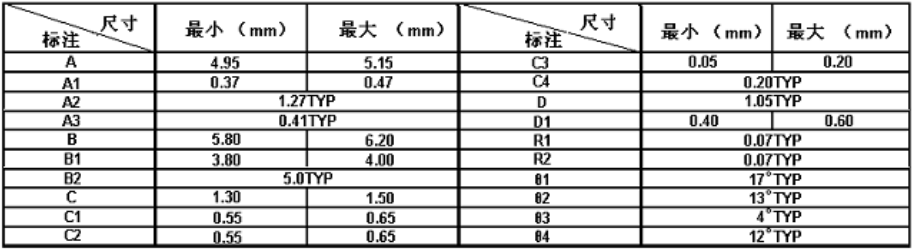
\includegraphics[width=1\textwidth]{fig99.png}
    \label{fig:fig99}
\end{figure}

\begin{figure}[h]
    \centering
    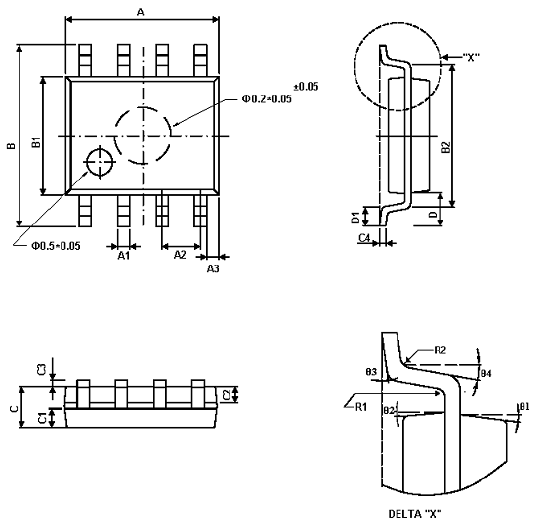
\includegraphics[width=1\textwidth]{fig11.png}
    \caption{Chip SOP8 Package Size Information}
    \label{fig:fig11}
\end{figure}

\end{document}
